\chapter{Numerical Experiments}


\section{Linear Model}\label{sec:num1}

In this section, we present numerical results.

\subsection{Implementational details and Hyperparameter choice}

We recall that all methods fall into the framework of either \eqref{eq: aatp counts} or \eqref{eq: aatp surrogate}. Since the threshold~$t$ depends on the weights~$\bm{w}$, we can consider the decision variable to be only~$\bm{w}$. Then to apply a method, we implemented the following iterative procedure. At iteration~$j$, we have the weights~$\bm{w}^j$ to which we compute the threshold~$t^j=t(\bm{w}^j)$. Then according to \eqref{eq:derivatives}, we compute the gradient of the objective and apply the ADAM descent scheme~\cite{kingma2014adam}. All methods were run for~$10000$ iterations using the stochastic gradient descent. The minibatch size was~$512$ except for the sigillito1989classification and Spambase datasets where the full gradient was used. All methods used the hinge surrogate \eqref{eq:defin_surrogate}. The initial point is generated randomly.

We run the methods for the following hyperparameters
\begin{equation}\label{eq:beta1}
  \begin{aligned}
    \beta   & \in  \{0.0001,\ 0.001,\ 0.01,\ 0.1,\ 1,\ 10\}, \\
    \lambda & \in \{0,\ 0.00001,\ 0.0001,\ 0.001,\ 0.01,\ 0.1\}, \\
    k       & \in \{1, 3, 5, 10, 15, 20\}.
  \end{aligned}
\end{equation}
For \TopPushK, \PatMat and \PatMatNP we fixed~$\lambda=0.001$ to have six hyperparameters for all methods. For all datasets, we choose the hyperparameter which minimized the criterion on the validation set. The results are computed on the testing set which was not used during training the methods.

\TopPush and \tauFPL were originally implemented in the dual. However, to allow for the same framework and the stochastic gradient descent, we implemented it in the primal. These two approaches are equivalent.

\subsection{Dataset description and Performance criteria}\label{sec:datasets}

For the numerical results, we considered 10 datasets summarized in Table~\ref{tab:counts}. They can be downloaded from the UCI repository. sigillito1989classification~\cite{sigillito1989classification} and Spambase are small, baldi2016parameterized~\cite{baldi2016parameterized} contains a large number of samples while guyon2005result~\cite{guyon2005result} contains a large number of features. We also considered six visual recognition datasets: MNIST, FashionMNIST, CIFAR10, CIFAR20, CIFAR100 and SVHN2. MNIST and FashionMNIST are grayscale datasets of digits and fashion items, respectively. CIFAR100 is a dataset of coloured images of items grouped into 100 classes. CIFAR10 and CIFAR20 merge these classes into 10 and 20 superclasses, respectively. SVHN2 contains coloured images of house numbers. As Table~\ref{tab:counts} shows, these datasets are imbalanced.

Each of the visual recognition datasets was converted into ten binary datasets by considering one of the classes~$\{0,\dots,9\}$ as the positive class and the rest as the negative class. The experiments were repeated ten times for each dataset from different seeds, which influenced the starting point and minibatch creation. We use tpr@fpr as the evaluation criterion. This describes the true-positive rate at a prescribed true-negative rate, usually of~$1\%$ or~$5\%$. For the linear classifier~$\bm{w}^\top \bm{x} - t$, it selects the threshold~$t$ so that the desired true-negative rate is satisfied and then computes the true-positive rate for this threshold.

\begin{table}[!ht]
  \centering
  \begin{tabular}{@{}lllllllll@{}}
    \toprule
    &  & \multicolumn{2}{c}{Training} & \multicolumn{2}{c}{Validation} & \multicolumn{2}{c}{Testing} \\ \cmidrule(lr){3-4} \cmidrule(lr){5-6} \cmidrule(l){7-8} 
    & $m$ & $n$ & $\frac{\npos}{n}$ & $n$ & $\frac{\npos}{n}$ & $n$ & $\frac{\npos}{n}$ \\ \midrule
    Ionosphere
      & $34$
      & $175$ & $36.0\%$ & $88$ & $36.4\%$ & $88$ & $35.2\%$ \\
    Spambase
      & $57$
      & $2300$ & $39.4\%$ & $1150$ & $39.4\%$ & $1151$ & $39.4\%$ \\
    Gisette
      & $5000$
      & $1000$ & $50.0\%$ & $1500$ & $50.0\%$ & $500$ & $50.0\%$ \\
    Hepmass
      & $28$
      & $5250000$ & $50.0\%$ & $1750000$ & $50.0\%$ & $3500000$ & $50.0\%$ \\
    MNIST
      & $28 \times 28 \times 1$
      & $44999$ & $11.2\%$ & $15001$ & $11.2\%$ & $10000$ & $11.4\%$ \\
    FashionMNIST
      & $28 \times 28\times 1$
      & $45000$ & $10.0\%$ & $15000$ & $10.0\%$ & $10000$ & $10.0\%$ \\
    CIFAR10
      & $32\times 32\times 3$
      & $37500$ & $10.0\%$ & $12500$ & $10.0\%$ & $10000$ & $10.0\%$ \\
    CIFAR20
      & $32 \times 32\times 3$
      & $37500$ & $5.0\%$ & $12500$ & $5.0\%$ & $10000$ & $5.0\%$ \\
    CIFAR100
      & $32 \times 32\times 3$
      & $37500$ & $1.0\%$ & $12500$ & $1.0\%$ & $10000$ & $1.0\%$ \\
    SVHN2
      & $32 \times 32\times 3$
      & $54944$ & $18.9\%$ & $18313$ & $18.9\%$ & $26032$ & $19.6\%$ \\
    \bottomrule
  \end{tabular}
  \caption{Structure of the used datasets. The training, validation and testing sets show the number of features~$m$, samples~$n$ and the fraction of positive samples~$\frac{\npos}{n}$.}
  \label{tab:counts}
\end{table}

\subsection{Numerical results}

Figure~\ref{fig:ptau} presents the standard ROC (receiver operating characteristic) curves on selected datasets. Since all methods from this paper are supposed to work at low false-positive rates, the~$x$ axis is logarithmic. Both figures depict averages over ten runs with different seeds. The left column depicts CIFAR100 while the right one Hepmass. These are the two more complicated datasets. We selected four representative methods: \PatMat and \PatMatNP as our methods and \TopPush and \tauFPL as state-of-the-art methods. Even though all methods work well, \PatMatNP seems to outperform the remaining methods on most levels of false-positive rate.

\begin{figure}[!ht]
  \centering
  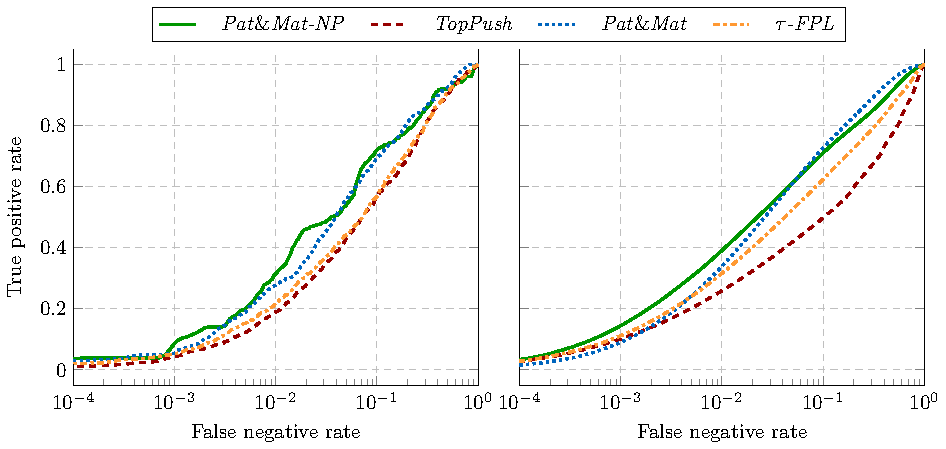
\includegraphics[width = \linewidth]{images/primal_results.pdf}
  \caption{ROC curves (with logarithmic~$x$ axis) on CIFAR100 (left) and Hepmass (right).}
  \label{fig:ptau}
\end{figure}

While Figure~\ref{fig:ptau} gave a glimpse of the behaviour of methods, Figures~\ref{fig:cd1} and~\ref{fig:cd2} provide a statistically more sound comparison. It employs the Nemenyi post hoc test for the Friedman test recommended in~\cite{demvsar2006statistical}. This test compares if the mean ranks of multiple methods are significantly different.

We consider 14 methods (we count different values of~$\tau$ as different methods) as depicted in this table. For each dataset mentioned in Section~\ref{sec:datasets} and each method, we evaluated the fpr@tpr metric and ranked all methods. Rank 1 refers to the best performance for given criteria, while rank 14 is the worst. The~$x$-axis shows the average rank over all datasets. The Nemenyi test computes the critical difference. If two methods are within their critical difference, their performance is not deemed to be significantly different. Black wide horizontal lines group such methods.

\begin{figure}[!ht]
  \centering
  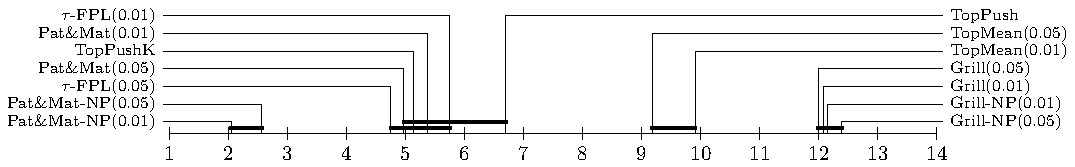
\includegraphics[width = \linewidth]{images/crit_diag_fpr_1.pdf}
  \caption{Critical difference (CD) diagrams (level of importance 0.05) of the Nemenyi post hoc test for the Friedman test. Each diagram shows the mean rank of each method, with rank 1 being the best. Black wide horizontal lines group together methods with the mean ranks that are not significantly different. The critical difference diagrams were computed for mean rank averages over all datasets of the tpr@fpr ($\tau=0.01$) metric.}
  \label{fig:cd1}
\end{figure}

\begin{figure}[!ht]
  \centering
  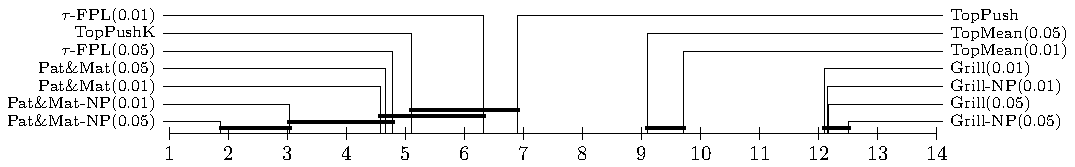
\includegraphics[width = \linewidth]{images/crit_diag_fpr_5.pdf}
  \caption{Critical difference (CD) diagrams (level of importance 0.05) of the Nemenyi post hoc test for the Friedman test. Each diagram shows the mean rank of each method, with rank 1 being the best. Black wide horizontal lines group together methods with the mean ranks that are not significantly different. The critical difference diagrams were computed for mean rank averages over all datasets of the tpr@fpr ($\tau=0.05$) metric.}
  \label{fig:cd2}
\end{figure}

From this figure and table, we make several observations:
\begin{itemize}
  \item \TopPushK (rank 5.1) provides a slight improvement over \TopPush (rank 6.7) even though this improvement is not statistically significant as both methods are connected by the black line in both Figures~\ref{fig:cd1} and~\ref{fig:cd2}.
  \item Neither \Grill (ranks 12.0 and 12.1) nor \GrillNP (ranks 12.1 and 12.4) perform well. We believe this happened due to the lack of convexity as indicated in Theorem~\ref{thm:convex} and the discussion after that.
  \item \TopMeanK (ranks 9.2 and 9.9) does not perform well either. Since the thresholds~$\tau$ are small, then~$\bm{w}=0$ is the global minimum as proved in Corollary~\ref{cor:topmean}.
  \item \PatMatNP (rank 2.1 and 2.6) seems to outperform other methods.
  \item \PatMat (ranks 5.0 and 5.4), \tauFPL (ranks 4.8 and 5.8) and \TopPushK (rank 5.1) perform similarly. Since they are connected, there is no statistical difference between their behaviours.
  \item \PatMatNP at level~$0.01$ (rank 2.1) outperforms \PatMatNP at level~$0.05$ (rank 2.6) for~$\tau=0.01$. \PatMatNP at level~$0.05$ (rank 1.9 in Figure~\ref{fig:cd2}) outperforms \PatMatNP at level~$0.01$ (rank 3.0 in Figure~\ref{fig:cd2}) for~$\tau=0.05$. This should be because these methods are optimized for the corresponding threshold. For~$\tauFPL$ we observed this behaviour for Figure~\ref{fig:cd2} but not for Figure~\ref{fig:cd1}.
\end{itemize}

Figure~\ref{fig:wilcoxon} provides a similar comparison. Both axes are sorted from the best (left) to the worst (right) average ranks. The numbers in the graph show the~$p$-value for the pairwise Wilcoxon signed-rank test, where the null hypothesis is that the mean tpr@fpr of both methods is the same. Even though Figure~\ref{fig:cd1} employs a comparison of mean ranks and Figure~\ref{fig:wilcoxon} a pairwise comparison of fpr@tpr, the results are almost similar. Methods grouped by the black line in the former figure usually show a large~$p$-value in the latter figure.

\begin{figure}[!ht]
  \centering
  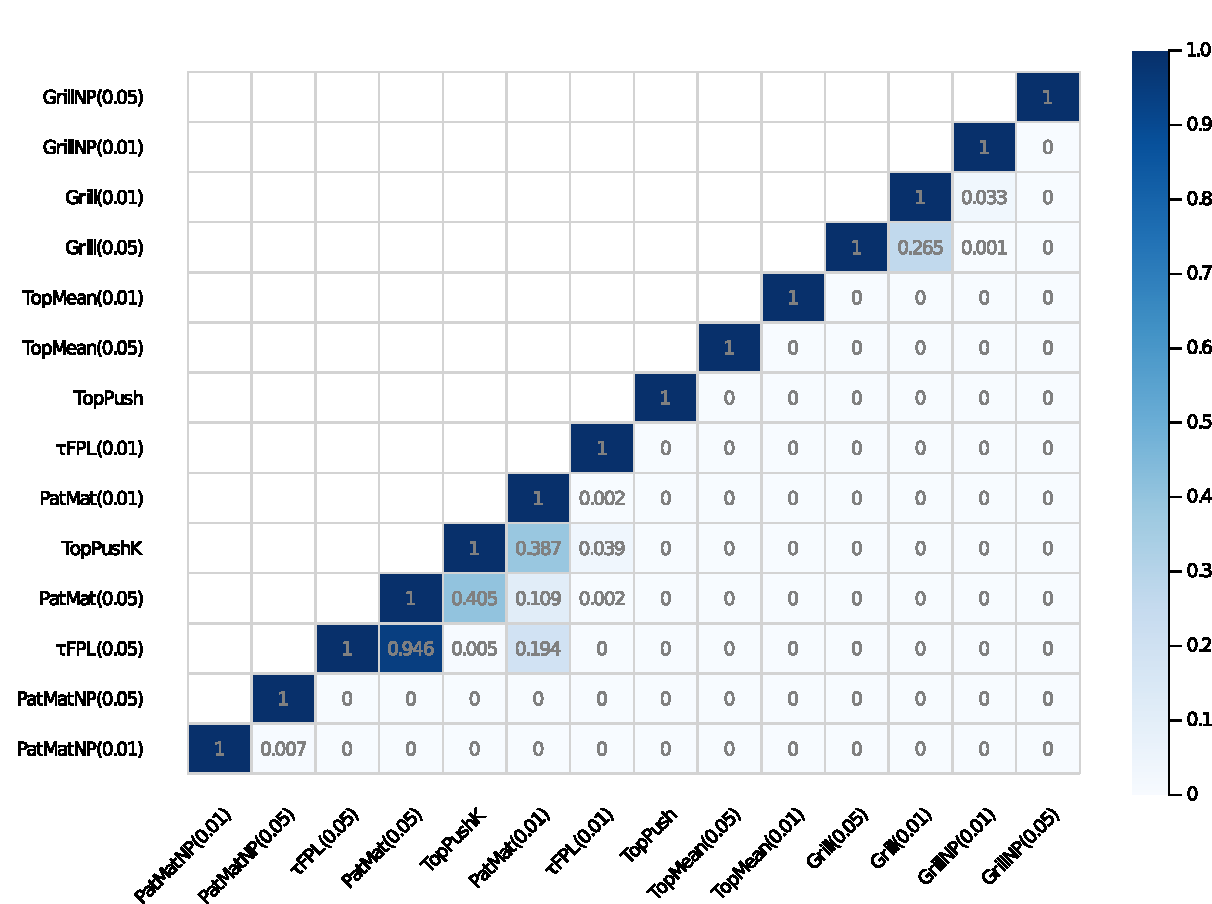
\includegraphics[width = \linewidth]{images/wilcoxon_fpr_1.pdf}
  \caption{The~$p$-value for the parwise Wilcoxon signed-rank test, where the null hypothesis is that the mean tpr@fpr(0.01) of both methods is the same. The methods are sorted by mean rank (left = better).}
  \label{fig:wilcoxon}
\end{figure}

Table~\ref{tab:fails} investigates the impact of~$\bm{w}=0$ as a potential global minimum. Each method was optimized for six different values of hyperparameters. The table depicts the condition under which the final value has a lower objective than~$\bm{w}=0$. Thus, \yesmark\ means that it is always better while \nomark\ means that the algorithm made no progress from the starting point~$\bm{w} =0$. The latter case implies that~$\bm{w}=0$ seems to be the global minimum. We make the following observations:
\begin{itemize}
  \item \PatMat and \PatMatNP are the only methods which succeeded at every dataset for some hyperparameter. Moreover, for each dataset, there was some~$\beta_0$ such that these methods were successful if and only if~$\beta\in(0,\beta_0)$. This is in agreement with Theorem~\ref{thm:patmat_zero}.
  \item \TopMeanK fails everywhere which agrees with Corollary~\ref{cor:topmean}.
  \item Figure~\ref{fig:thresholds} states that the methods from Section~\ref{sec: aatp} has a higher threshold than their Neyman-Pearson variants from Section~\ref{sec: Neyman-Pearson}. This is documented in the table as the latter have a higher number of successes.
\end{itemize}

\begin{table}[!ht]
  \centering
  \begin{tabular}{@{}lllll@{}}
    \toprule
    & Ionosphere & Hepmass & FashionMNIST & CIFAR100 \\
    \midrule
    \TopPush
      & \yesmark & \nomark & \yesmark & \nomark \\
    \TopPushK
      & \yesmark & \nomark & \yesmark & \nomark \\
    \Grill$\tau=0.01$
      & \nomark & \nomark & \nomark & \nomark \\
    \phantom{\Grill}$\tau=0.05$
      & \nomark &\nomark & \nomark & \nomark \\
    \PatMat$\tau=0.01$
      & \yesmark & \good{\boldmath$\beta\le 0.1$} & \good{\boldmath$\beta\le 1$} & \good{\boldmath$\beta\le 1$} \\
    \phantom{\PatMat}$\tau=0.05$
      & \yesmark & \good{\boldmath$\beta\le 1$} & \yesmark & \yesmark \\
    \TopMeanK$\tau=0.01$
      & \nomark & \nomark & \nomark & \nomark \\
    \phantom{\TopMeanK}$\tau=0.05$
      & \nomark & \nomark & \nomark & \nomark \\
    \GrillNP$\tau=0.01$
      & \nomark & \nomark & \nomark & \nomark \\
    \phantom{\GrillNP}$\tau=0.05$
      & \nomark & \nomark & \nomark & \nomark \\
    \PatMatNP$\tau=0.01$
      & \yesmark & \good{\boldmath$\beta\le 1$} & \yesmark & \good{\boldmath$\beta\le 1$} \\
    \phantom{\PatMatNP}$\tau=0.05$
      & \yesmark & \yesmark & \yesmark & \good{\boldmath$\beta\le 1$} \\
    \tauFPL$\tau=0.01$
      & \yesmark & \nomark & \yesmark & \nomark \\
    \phantom{\tauFPL}$\tau=0.05$
      & \yesmark & \yesmark & \yesmark & \good{\boldmath$\lambda\le 0.001$} \\
    \bottomrule
  \end{tabular}
  \caption{Necessary hyperparameter choice for the solution to have a better objective than zero. \yesmark\ means that the solution was better than zero for all hyperparameters while \nomark\ means that it was worse for all hyperparameters.}
  \label{tab:fails}
\end{table}


\section{Dual}\label{sec:Numerical experiments}

In this section, we present numerical results. All codes were implemented in the Julia language~\cite{bezanson2017julia} and are available online.\footnote{All codes are available at \url{https://github.com/VaclavMacha/ClassificationOnTop_new.jl}}

\subsection{Performance criteria}

For the evaluation of numerical experiments, we use precision and recall. For a threshold~$t$ they are defined by
\begin{equation}\label{eq:prec_rec}
  \begin{alignedat}{2}
      \precision
      & = \frac{\sum_{i = 1}^{\npos} [\bm{w}^{\top}\bm{x}^+_{i} - t]}{\sum_{i = 1}^{n} [\bm{w}^{\top}\bm{x}_{i} - t]}, & \qquad
      \recall
      & = \frac{1}{\npos} \sum_{i = 1}^{\npos} [\bm{w}^{\top}\bm{x}^+_{i} - t].
  \end{alignedat}
\end{equation}
We also use the Precision-Recall (PR) curve that are commonly used for unbalanced data~\cite{davis2006relationship} and precision at a certain level of recall which we denote by~$\pratrec$.

\subsection{Hyperparameter choice}

In Section~\ref{sec:New method for solving dual problems} we introduced Algorithm~\ref{alg:Coordinate descent} for solving dual problems~(\ref{eq: TopPushK dual},~\ref{eq: PatMat dual}). We let it run for~$20000$ \repeatloop loops, which corresponds to~$40000$ updates of coordinates of~$(\bm{\alpha},\bm{\beta})$. We use the linear and Gaussian kernels defined by
\begin{align}
  k_{\textrm{lin}}(\bm{x}, \bm{y})   & = \bm{x}^{\top} \bm{y}, \label{eq:Linear kernel} \\
  k_{\textrm{gauss}}(\bm{x}, \bm{y}) & = \exp\{-\sigma \norm{\bm{x} - \bm{y}}_2^2\} \label{eq:Gaussian kernel}
\end{align}
and the truncated quadratic loss~\eqref{eq:Truncated quadratic loss} with~$\vartheta = 1$ as a surrogate. 

The classifiers were trained on the training set. We selected the optimal hyperparameter from
\begin{equation*}
  \begin{aligned}
    \tau   & \in \{0.01,\ 0.05,\ 0.1\}, &
    K      & \in \{5,\ 10\}, &
    C      & \in \{0.1,\ 1,\ 10\}, &
    \sigma & \in \{0.01,\ 0.05\} 
  \end{aligned}
\end{equation*}
which gave the best performance on the validation set. All presented result are shown on the testing set which was not part of the training process.

\begin{table}[ht]
  \centering
  \begin{tabular}{@{}lllllllll@{}}
      \toprule
      &&& \multicolumn{2}{c}{Training}
        & \multicolumn{2}{c}{Validation}
        & \multicolumn{2}{c}{Testing} \\
      \cmidrule(lr){4-5} \cmidrule(lr){6-7} \cmidrule(l){8-9}
        & $y^+$
        & $d$
        & $n$
        & $\frac{\npos}{n}$
        & $n$
        & $\frac{\npos}{n}$
        & $n$
        & $\frac{\npos}{n}$ \\
      \midrule
      sigillito1989classification
        & -- & 34 & 176 & 64.2\% & 87 & 64.4\% & 88 & 63.6\% \\
      Spambase
        & -- & 57 & 2301 & 39.4\% & 1150 & 39.4\% & 1150 & 39.4\% \\
      WhiteWineQuality
        & 7, 8, 9 & 11 & 2449 & 21.6\% & 1224 & 21.7\% & 1225 & 21.6\% \\
      RedWineQuality
        & 7, 8 & 11 & 800 & 13.5\% & 400 & 13.8\% & 399 & 13.5\% \\
      Fashion-MNIST
        & 0 & 784 & 50000 & 10.0\% & 10000 & 10.0\% & 10000 & 10.0\% \\
      \bottomrule
  \end{tabular}
  \caption{Summary of the used datasets. It shows which original labels~$y^+$ were selected as the positive class, the number of features~$d,$ samples~$n,$ and the fraction of positive samples~$\frac{\npos}{n}$.}
  \label{tab:Datasets}
\end{table}

\subsection{Dataset description}

For numerical experiments, we consider the FashionMNIST dataset~\cite{xiao2017fashionmnist} and four smaller datasets from the UCI repository~\cite{dua2019uci}: sigillito1989classification~\cite{sigillito1989classification}, Spambase, WhiteWineQuality~\cite{cortez2009modeling} and RedWineQuality~\cite{cortez2009modeling}. Datasets that do not contain testing set were randomly divided into a training (50\%), validation (25\%) and testing (25\%) sets. For datasets that contain a testing set, the training set was randomly divided into a training and a validation set, where the validation set has the same size as the testing set. FashionMNIST dataset was converted to binary classification tasks by selecting class with label 0 as the positive class and the rest as the negative class. All datasets are summarized in Table~\ref{tab:Datasets}.

\subsection{Experiments}

In Figure~\ref{fig:PR comparison} we present the PR curves for all methods with two different kernels evaluated on the FashionMNIST dataset. The left column corresponds to the linear kernel~\eqref{eq:Linear kernel} while the right one to the Gaussian kernel~\eqref{eq:Gaussian kernel} with~$\sigma = 0.01$. The nonlinear Gaussian kernel significantly outperforms the linear kernel. This will be confirmed later in Table~\ref{tab:Metrics comparison} where we present a comparison from multiple datasets. 

\begin{figure}[!ht]
  \centering
  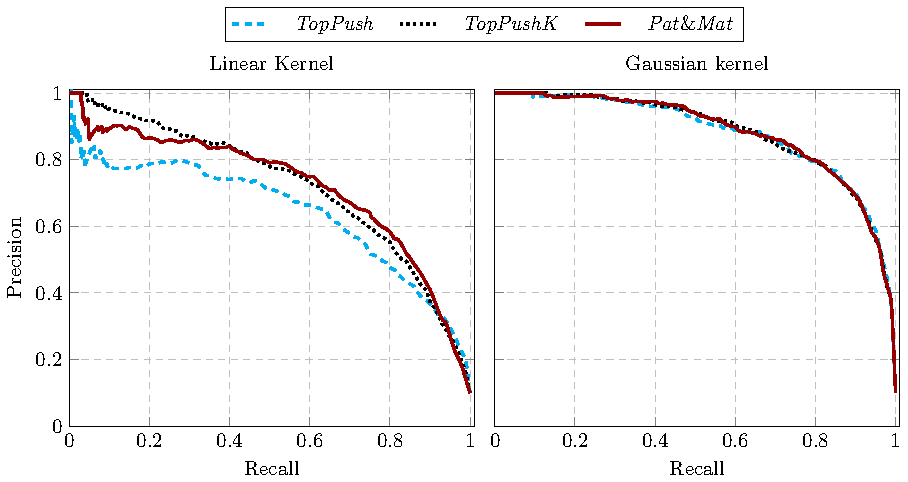
\includegraphics[width = \linewidth]{images/dual_results1.pdf}
  \caption{PR curves for all methods and  FashionMNIST dataset. The left column corresponds to the linear kernel~\eqref{eq:Linear kernel} and the right column corresponds to the Gaussian kernel~\eqref{eq:Gaussian kernel}.}
  \label{fig:PR comparison}
\end{figure}

For a better illustration of how the methods from Figure~\ref{fig:PR comparison} work, we present density estimates of scores~$\bm s$ from \eqref{eq:defin_s}. High scores predict positive labels while low scores predict negative labels. The rows of Figure~\ref{fig:Scores comparison} depict the linear \eqref{eq:Linear kernel} and the Gaussian kernels \eqref{eq:Gaussian kernel} with~$\sigma = 0.01$ while each column corresponds to one method. The black vertical lines depict the top 5\%-quantile of all scores (on the testing set). Since a smaller overlap of scores of samples with positive and negative labels implies a better separation, we deduce the benefit of the Gaussian over the linear kernel.

\begin{figure}[!ht]
  \centering
  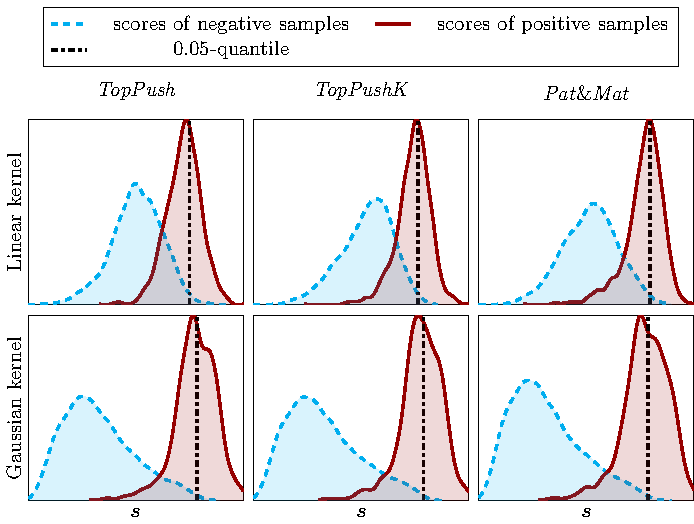
\includegraphics[width = \linewidth]{images/dual_results2.pdf}
  \caption{Density estimates for scores corresponding to samples with positive and negative labels for the FashionMNIST dataset.}
  \label{fig:Scores comparison}
\end{figure}

In Table~\ref{tab:Metrics comparison} we present the precision of all methods across all datasets from Table~\ref{tab:Datasets}. For each dataset, we trained each method and computed precision at certain levels of recall. The depicted values are averages over all datasets. For each kernel and each level of recall, the best precision is highlighted in light green. Moreover, the best overall precision for each level of recall is depicted in dark green. We can make several observations from Table~\ref{tab:Metrics comparison}:
\begin{itemize}
  \item All methods perform better with the Gaussian kernels than with the linear kernel. 
  \item \TopPush and \TopPushK perform better for sufficiently small recall. This happened because they consider the threshold to be the maximal~$K$ negative scores and small recall corresponds to high threshold. However, for the same reason, \TopPush is not robust.
  \item \PatMat is the best for all kernels if the recall is sufficiently large. The reason is again the form of the decision threshold.
\end{itemize}

\begin{table}[ht]
  \centering
  \begin{tabular}{@{}c|llllllll@{}}
    \toprule
    \multicolumn{3}{c}{} & \multicolumn{6}{c}{$\pratrec$}  \\
    \cmidrule(lr){4-9}
    \multicolumn{3}{c}{}
      & 0.05 & 0.1 & 0.2 & 0.4 & 0.6 & 0.8 \\
    \midrule
    \multirow{6}{*}{\rotatecell{Linear kernel}}
    & \TopPush
      & & \best 79.83 & 64.27 & \best 65.55 & 61.85 & 57.89 & 51.83 \\
    & \TopPushK & $K = 5$
      & 73.96 & \best 65.41 & 64.82 & 60.28 & 56.94 & 50.52 \\
    & & $K = 10$
      & 60.63 & 61.97 & 59.69 & 56.89 & 54.40 & 49.83 \\
    & \PatMat & $\tau = 0.01$
      & 63.67 & 60.30 & 58.74 & 57.75 & 53.32 & 48.42 \\
    & & $\tau = 0.05$
      & 54.05 & 60.91 & 63.32 & 55.24 & 52.55 & 48.30 \\
    & & $\tau = 0.1$
      & 57.02 & 61.24 & 62.49 & \best 63.11 & \best 59.91 & \best 52.14 \\
    \midrule
    \multirow{6}{*}{\rotatecell{Gaussian kernel}}
    & \TopPush
      & & \besttotal 97.50 & 86.06 & 81.28 & 76.15 & 71.13 & 60.17 \\
    & \TopPushK & $K = 5$
      & 92.50 & 87.56 & 85.31 & 78.47 & 70.77 & 57.10 \\
    & & $K = 10$
      & 89.50 & 87.56 & 83.15 & 79.09 & 71.88 & 59.27 \\
    & \PatMat & $\tau = 0.01$
      & 89.65 & \besttotal 89.11 & \besttotal 86.75 & 80.77 & 75.44 & 65.95 \\
    & & $\tau = 0.05$
      & 80.77 & 81.28 & 85.74 & 82.92 & 74.91 & 65.04 \\
    & & $\tau = 0.1$
      & 81.30 & 84.14 & 82.58 & \besttotal 83.12 & \besttotal 77.82 & \besttotal 66.50 \\
    \bottomrule
  \end{tabular}
  \caption{The precision of all methods averaged across all datasets from Table~\ref{tab:Datasets}. Each column represents precision at a certain level of recall. Light green depicts the best method for the given kernel and dark green depicts the best overall method.}
  \label{tab:Metrics comparison}
\end{table}

In Figure~\ref{fig:Convergence comparison}, we investigate the convergence of methods. In each column, we show the convergence of primal and dual problems for one method. To solve the primal problem, we use the gradient method proposed in~\cite{adam2021general}. For the dual problem, we use our Algorithm~\ref{alg:Coordinate descent}. Since~\cite{adam2021general} considers only linear kernels, we present them. Moreover, since the computation of the objective is expensive, the results are presented for the sigillito1989classification dataset. We can see that \TopPush and \TopPushK converge to the same objective for primal and dual problems. This means that the problem was solved to optimality. However, there is a little gap between optimal solution of primal and dual problems for \PatMat.

\begin{figure}[!ht]
  \centering
  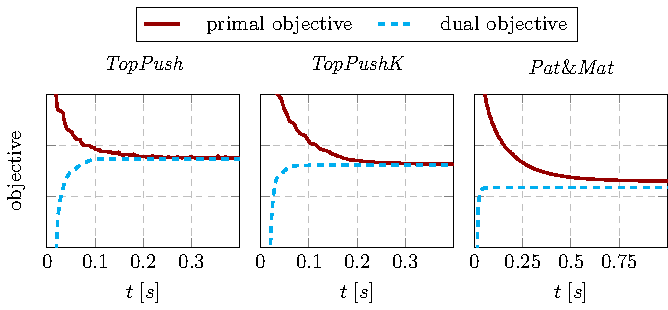
\includegraphics[width = \linewidth]{images/dual_results3.pdf}
  \caption{Convergence of the objectives for the primal (red line) and dual (blue line) problems for the sigillito1989classification dataset with linear kernel.}
  \label{fig:Convergence comparison}
\end{figure}

Finally, Table~\ref{tab:Time comparison} depicts the time comparison for all methods and all datasets. It shows the average time in milliseconds needed for one \repeatloop loop in Algorithm~\ref{alg:Coordinate descent}. The time is relatively stable and for most of the datasets it is below one millisecond. Since we run all experiments for 20000 \repeatloop loops, the evaluation of one method with one hyperparameter setting takes a few seconds for smaller datasets and approximately 7 minutes for FashionMNIST. The average time for one~$\Delta_l$ in step~\ref{alg: line 5} in Algorithm~\ref{alg:Coordinate descent} took between~$1.7\cdot 10^{-7}$ and~$3.1\cdot 10^{-7}$ seconds for each methods. It is almost the same for all datasets, which corresponds to the fact that the complexity of step~\ref{alg: line 5} is independent of the size of the dataset. Note that in all experiments we used precomputed kernel matrix~$\K$ saved on the hard drive and not in memory.

\begin{table}[ht]
  \centering
  \begin{tabular}{@{}c|llll@{}}
      \toprule
      \multicolumn{2}{c}{}
        & \TopPush & \TopPushK & \PatMat \\
      \midrule
      \multirow{5}{*}{\rotatecell{One \repeatloop \\ loop [ms]}}
      & sigillito1989classification
        & $ 0.04 \pm 0.00 $ & $ 0.03 \pm 0.00 $ & $ 0.03 \pm 0.00 $ \\
      & Spambase
        & $ 0.56 \pm 0.02 $ & $ 0.49 \pm 0.01 $ & $ 0.50 \pm 0.01 $ \\
      & WhiteWineQuality
        & $ 0.62 \pm 0.03 $ & $ 0.53 \pm 0.01 $ & $ 0.54 \pm 0.01 $ \\
      & RedWineQuality
        & $ 0.17 \pm 0.01 $ & $ 0.14 \pm 0.01 $ & $ 0.15 \pm 0.01 $ \\
      & Fashion-MNIST
        & $ 17.16 \pm 0.74 $ & $ 15.95 \pm 0.14 $ & $ 15.54 \pm 0.80 $ \\
      \bottomrule
  \end{tabular}
  \caption{The average time with standard deviation (in milliseconds) for one \repeatloop loop in Algorithm~\ref{alg:Coordinate descent}. The average time for one~$\Delta_l$ in step~\ref{alg: line 5} in Algorithm~\ref{alg:Coordinate descent} took between~$1.7\cdot 10^{-7}$ and~$3.1\cdot 10^{-7}$ seconds for each methods.}
  \label{tab:Time comparison}
\end{table}


\section{Neural Networks}\label{sec:numerics}

This section presents numerical results for \DeepTopPush. Table~\ref{table:summary} shows that it is similar to \PatMatNP. While the former maximizes the number of positives above the largest negative, while the latter maximizes the number of positives above the~$\nneg\tau$-largest negative. The former may be understood as requiring no false-positives, while the latter allows for false positive rate~$\tau$.

Section~\ref{sec:bias1} showed that we can use large minibatches to obtain good results for \PatMatNP for small fractions of top samples~$\tau$. Section~\ref{sec:bias2} showed that \DeepTopPush works well even with small minibatches if we track the threshold by enhancing the minibatch by one sample. We present numerical comparisons in several sections, each with a different purpose. Comparison with the prior art \TFCO and \APPerf is performed on several visual recognition datasets and shows that \DeepTopPush outperforms other methods. Then we present two real-world applications. The first one shows that \DeepTopPush can handle ranking problems. The second one presents results on a complex malware detection problem. Finally, we show similarities between \DeepTopPush and \PatMatNP and explain why enhancing the minibatch in Algorithm~\ref{alg2} works.

\subsection{Dataset description and Computational setting}\label{sec:set}

We consider the following image recognition datasets: FashionMNIST~\cite{xiao2017fashionmnist}, CIFAR100~\cite{krizhevsky2009learning}, SVHN2~\cite{netzer2011reading} and ImageNet~\cite{russakovsky2015imagenet}. These datasets were converted to binary classification tasks by selecting one class as the positive class and the rest as the negative class. ImageNet merged turtles and non-turtles. We also consider the 3A4 dataset~\cite{ma2015deep} with molecules and their activity levels. Finally, malware analysis reports of executable files were provided by a cybersecurity company. This is an extremely tough dataset as individual samples are JSON files whose size ranges from 1kB to 2.5MB. Moreover, they contain different features, and their features may have variable lengths. All datasets are summarized in the appendix.

We use truncated quadratic loss~$l(z) = (\max\{0, 1 + z\})^2$ as the surrogate function and~$\tau=\frac{1}{\nneg}$ and~$\tau=0.01$. This first one computes the true positive rate above the second highest-ranked negative, while the latter allows for the false positive rate of~$1\%$. All algorithms were run for~$200$ epochs on an NVIDIA P100 GPU card with balanced minibatches of 32 samples. The only exception was Malware Detection, which was run on a cluster in a distributed manner, and where the minibatch size was~$20000$. For the evaluation of numerical experiments, we use the standard receiver operating characteristic (ROC) curve. All results are computed from the test set. All codes were implemented in the Julia language~\cite{bezanson2017julia}. The network structure was the same for all methods; we describe them in the online appendix.

\subsection{Comparison with prior art}\label{sec:comparison}

We compare our methods with \BaseLine, which uses the weighted cross-entropy. Moreover, we use two prior art methods which have codes available online, namely \TFCO~\cite{cotter2019optimization,narasimhan2019optimizing} and \APPerf~\cite{fathony2019ap}. We did not implement the original TopPush because its duality arguments restrict the classifiers to only linear ones. Table~\ref{table:time} shows the time requirement per epoch. All methods besides \APPerf have similar time requirements, while \APPerf is much slower. This difference increases drastically when the minibatch size increases, as noted in~\cite{fathony2019ap}. We do not present the results for SVHN for \APPerf because it was too slow and for \TFCO because we encountered a TensorFlow memory error. All these methods are designed to maximize true-positives when the false positive rate is at most~$\tau$. This is the same as for \PatMatNP.

\begin{table}[!ht]
  \centering
  \begin{tabular}{@{}llll@{}}
      \toprule      
       & FashionMNIST & CIFAR100 & SVHN \\
      \midrule
      BaseLine
        & 4.4s & 5.1s & 62.8s \\
      DeepTopPush
        & 4.8s & 5.6s & 66.6s \\
      Pat\&Mat-NP
        & 4.8s & 5.6s & 66.6s \\
      TFCO
        & 7.2s & 6.5s & - \\
      AP-Perf
        & 95.3s & 81.2s & - \\
      \bottomrule
  \end{tabular}
  \caption{Time requirements per epoch for investigated methods for minibatches of size~$\nmin=32$.}
  \label{table:time}
\end{table}

\begin{table}[ht]
  \centering
  \footnotesize
  \begin{tabular}{@{}c|llllll@{}}
    \toprule
    & \thead{Dataset}
    & \thead{BaseLine}
    & \thead{DeepTopPush}
    & \thead{Pat\&Mat-NP}
    & \thead{TFCO}
    & \thead{AP-Perf} \\
    \midrule
    \multirow{4}{*}{\rotatebox[origin=c]{90}{\parbox[c]{1.5cm}{\centering tpr@fpr $\tau=\nicefrac{1}{\nneg}$}}}
    & FashionMNIST
      & $5.06 \pm 1.41$
      & \best $27.30 \pm 5.91$
      & $22.21 \pm 5.62$
      & $11.30 \pm 3.44$
      & $9.90$ \\
    & CIFAR100
      & $1.70 \pm 0.46$
      & \best $14.40 \pm 5.44$
      & $8.10 \pm 3.45$
      & $7.70 \pm 2.28$
      & $5.00$ \\
    & 3A4
      & $2.58 \pm 0.61$ 
      & \best $5.61 \pm 1.70$
      & $3.79 \pm 0.90$
      & $3.03 \pm 1.52$
      & $3.03$ \\
    & SVHN
      & $6.51 \pm 1.37$
      & \best $12.21 \pm 5.39$
      & $12.07 \pm 4.41$ 
      & - & -\\
    \midrule
    \multirow{4}{*}{\rotatebox[origin=c]{90}{\parbox[c]{1.5cm}{\centering tpr@fpr $\tau=0.01$}}}
    & FashionMNIST
      & $63.14 \pm 1.39$
      & \best $75.37 \pm 1.18$
      & $74.11 \pm 1.00$
      & $73.27 \pm 2.92$
      & $64.60$ \\
    & CIFAR100
      & $49.40 \pm 4.90$
      & \best $70.20 \pm 2.14$
      & $66.30 \pm 2.33$
      & $67.30 \pm 1.79$
      & $65.00$ \\
    & 3A4
      & $57.80 \pm 0.35$ 
      & $60.08 \pm 3.35$
      & \best $65.91 \pm 0.59$
      & $54.55 \pm 10.22$
      & $63.64$ \\
    & SVHN
      & $84.72 \pm 0.84$
      & $91.05 \pm 1.45$
      & \best $91.07 \pm 0.30$
      & - & - \\
    \bottomrule
  \end{tabular}
  \caption{The true positive rates (in \%) at two levels of false positive rates averaged across ten indepenedent runs with standard deviation. The best methods are highlighted.}
  \label{tab:Overall comparison}
\end{table}

Table~\ref{tab:Overall comparison} shows the true positive rate (tpr) above the second-largest negative and at the prescribed false positive rate (fpr)~$\tau=0.01$. Using the second-largest negative, which corresponds to~$\tau=\frac{1}{\nneg}$, allows for one outlier. The results are averaged over ten independent runs except for AP-Perf, which is too slow. The best result for each metric (in columns) is highlighted. All methods are better than \BaseLine. This is not surprising as all these methods are designed to work well for low false positive rates. \DeepTopPush outperforms all other methods at the top, while it performs well at the low fpr of~$\tau=0.01$. There \PatMatNP, which also falls into our framework, performs well. Both these methods outperform the state of the art methods. 

Figure~\ref{fig: roc curves} \textbf{A)} shows the ROC curves on CIFAR100 averaged over ten independent runs. We use the logarithmic~$x$ axis to highlight low fpr modes. \DeepTopPush performs significantly the best again whenever the false positive rate is smaller than~$0.01$.

As a further test, we performed a simple experiment on ImageNet. We modified the pre-trained EfficientNet B0~\cite{tan2019efficientnet} by removing the last dense layer and adding another dense layer with one output. Then we retrained the newly added layer to perform well at the top. The original EfficientNet achieved~$68.0\%$ at the top, while \DeepTopPush achieved~$70.0\%$ for the same metric. This shows that \DeepTopPush can provide better accuracy at the top than pre-trained networks.

\subsection{Application to ranking}

The 3A4 dataset contains information about activity levels of approximately~$50000$ molecules, each with about~$10000$ descriptors. The activity level corresponds to the usefulness of the molecule for creating new drugs. Since medical scientists can focus on properly investigating only a small number of molecules, it is important to select a small number of molecules with high activity.

We converted the continuous activity level into binary by considering a threshold on the activity. Since the input is large-dimensional, and there is no spatial structure to use convolutional neural networks, we used PCA to reduce the dimension to~$100$. Then we created a network with two hidden layers and applied \DeepTopPush to it. The test activity was evaluated at the continuous (and not binary level). Table~\ref{tab:Overall comparison} shows again the results at the top. \DeepTopPush outperforms other methods. Figure~\ref{fig:molecules} shows that high scores (output of the network) indeed correspond to high activity. Thus, even though the problem was ``binarized'' and its dimension reduced, our algorithm was able to select a small number of molecules with high activity levels. These molecules can be used for further manual (expensive) investigation.

\begin{figure}[!ht]
  \centering
  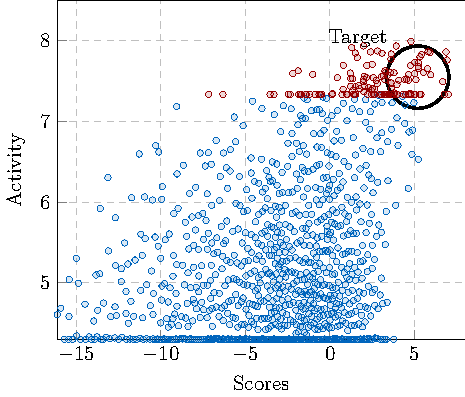
\includegraphics[width = \linewidth]{images/deep_molecules.pdf}
  \caption{Results for the 3A4 dataset. The goal was to assign large scores to a few molecules with high activity (scores on top-right are preferred).}
  \label{fig:molecules}
\end{figure}

\begin{figure*}[!ht]
  \centering
  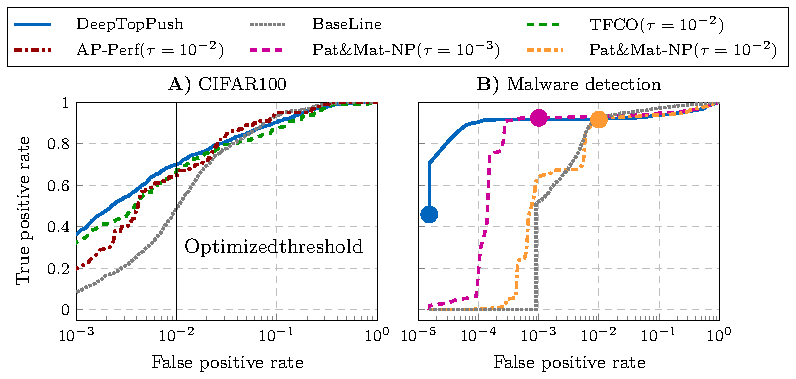
\includegraphics[width = \linewidth]{images/deep_results1.pdf}
  \caption{\textbf{A)} ROC curves averaged over ten runs on the CIFAR100 dataset. \textbf{B)} ROC curve for Malware Detection dataset. The circles show the thresholds the methods were optimized for.}
  \label{fig: roc curves}
\end{figure*}

\subsection{Real-world application}

This section shows a real-world application of the accuracy at the top. A renowned cybersecurity company provided malware analysis reports of executable files. Its structure is highly complicated because each sample has a different number of features, and features may have a complicated structure, such as a list of ports to which the file connects. This is in sharp contrast with standard datasets, where each sample has the same number of features, and each feature is a real number. We processed the data by a public implementation of hierarchical multi-instance learning (HMIL)~\cite{pevny2017using}. Then we applied \DeepTopPush and \PatMatNP at~$\tau=10^{-3}$ and~$\tau=10^{-2}$. The latter maximizes the true positives rate when the false positive rate is at most~$\tau$. The minibatch size was~$20000$, which allowed us to obtain precise threshold estimates and unbiased sampled gradients due to Section~\ref{sec:bias1}.

Figure~\ref{fig: roc curves} \textbf{B)} shows the performance on the test set. \DeepTopPush is again the best at low false positive rates. This is extremely important in cybersecurity as it prevents false alarms for malware. Even at the extremely low false positive rate~$\tau=10^{-5}$, our algorithm correctly identified~$46\%$ of malware. The circles denote the thresholds for which the methods were optimized. \DeepTopPush should have the best performance at the leftmost point, \PatMatNP ($\tau=10^{-3}$) at~$\tau=10^{-3}$ and similarly \PatMatNP($\tau=10^{-2}$).

\subsection{Impact of enhancing the minibatch}\label{sec:delay}

The crucial aspect of \DeepTopPush is enhancing the minibatch by one sample. In all presented results with the exception of the Malware Detection, the minibatch contained only 32 samples. Then the discussion in Section~\ref{sec:bias2} implies that \PatMatNP equals to \DeepTopPush without enhancing the minibatch. In other words, \PatMatNP uses Algorithm~\ref{alg1} while \DeepTopPush uses Algorithm~\ref{alg2}. As Table~\ref{tab:Overall comparison} clearly shows that \DeepTopPush ourperforms \PatMatNP, this implies that using the delayed values is beneficial.

Figure~\ref{fig:thresholds2} shows explanation for this behaviour. The full blue line shows the behaviour of \DeepTopPush while the dotted grey line shows \PatMatNP. As explained in the previous paragraph, their difference demonstrates the effect of enhancing the minibatch by one delayed value. The top subfigure compares thresholds with the true threshold (dashed black). While the threshold for \PatMatNP jumps wildly, it is smooth for \DeepTopPush, and it often equals the true threshold. Theorem~\ref{theorem:convergence} then implies that our sampled gradient is an unbiased estimate of the true gradient. This is even more pronounced in the bottom subfigure, which shows the angle between the true gradient and the computed gradient. This angle is important because~\cite{nocedal2006numerical} showed that if this angle is uniformly in the interval~$[0,90)$, then gradient descent schemes converge. This is precisely what happened for \DeepTopPush. When the threshold is correct, the true and estimated gradients are parallel to each other, and the gradient descent moves in the correct direction.

\begin{figure}[!ht]
  \centering
  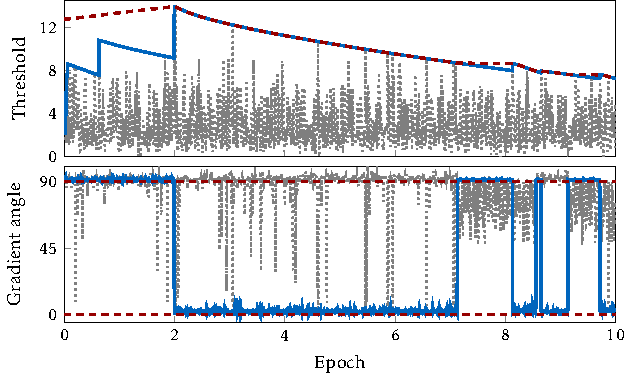
\includegraphics[width = \linewidth]{images/deep_thresholds.pdf}
  \caption{The thresholds (top) and angle between true and sampled gradients (bottom) for Algorithm~\ref{alg1} (full blue) and Algorithm~\ref{alg2} (dotted gray).}
  \label{fig:thresholds2}
\end{figure}